\documentclass{article} % say
\usepackage{tikz}
\renewcommand{\familydefault}{\sfdefault} % for sans font
\begin{document}


\texttt{Bitmap.Optimize()} uses the values of \texttt{c.n} (cardinality) and
\texttt{c.runCount()} to convert container types, achieving minimal storage size, according to this diagram:\\

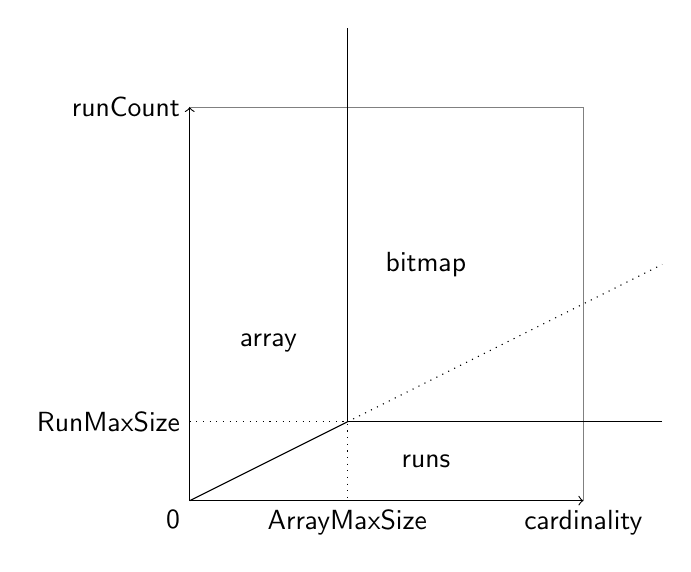
\begin{tikzpicture}
  \draw [<->] (0,5) node [left] {runCount} -- (0,0) node [below left] {0} -- (5,0) node [below] {cardinality};
  \draw [help lines] (5, 0) -- (5, 5) -- (0, 5);
  \draw [dotted] (0,1) node [left] {RunMaxSize} -- (2,1) -- (2,0) node [below] {ArrayMaxSize};
  \draw [solid] (6, 1) -- (2,1) -- (2,6);
  \draw [solid] (0, 0) -- (2, 1);
  \draw [dotted] (2, 1) -- (6, 3);
  \node at (1, 2) {array};
  \node at (3, .5) {runs};
  \node at (3, 3) {bitmap};
\end{tikzpicture}

\bigskip


Container elements are 16-bit values stored in \texttt{uint32}s. Array elements are
single values, runs are two values (start and end). Switching to \texttt{uint16}s
instead, which will save space for these container types.\\
\\
\begin{tabular}{l | c | c}
    & 32-bit & 16-bit \\
  \hline
  ArrayMaxSize & 2048 & 4096 \\
  \hline
  RunMaxSize & 1024 & 2048 \\
\end{tabular}

\end{document}

